
\section{Baseline: Temporal Replication and Parallel Mining}
\label{sec:trm}
In this section, we propose a baseline solution that resorts to MapReduce (MR) as a general, parallel and scalable paradigm for GCMP pattern mining. The framework, named \textit{temporal replication and parallel mining} (TRPM), is illustrated in   Figure~\ref{fig:trm}. There are two cycles of map-reduce jobs connected in a pipeline manner. The first cycle deals with spatial clustering in each snapshot, which can be seen as a preprocessing step for the subsequent pattern mining. In particular, the timestamp is treated as the key in the map phrase and objects within the same snapshot are clustered (DBSCAN or disk-based clustering) in the reduce phrase. Finally, the reducers output clusters of objects in each snapshot, represented by a list of $S_t$, where $t$ is the timestamp and $S_t$ is a set of clustered objects at snapshot $t$. 

Our focus in this paper is the second map-reduce cycle of parallel mining, which essentially consists of two key questions to solve. The first is how to employ effective data partitioning such that the mining can be conducted independently; and the second is how to efficiently mine the valid patterns within each partition. 


It is obvious that we cannot simply split the trajectory database into disjoint partitions because a GCMP pattern requires $L$-consecutive and the corresponding segments may cross multiple partitions. Our strategy is to use data replication to enable parallel mining. Each snapshot will replicate its clusters to $\eta$ preceding snapshots. In other words, the partition for the snapshot $S_t$ contains clusters in $S_t$, $S_{t+1}\ldots,S_{t+\eta}$. Determining a proper $\eta$ is critical in ensuring the
correctness and efficiency of TRPM. If $\eta$ is too small, certain cross-partition patterns may be missed. If $\eta$ is set too large, expensive network communication and CPU processing costs would be incurred in the map and reduce phrases respectively. 

To guarantee that no valid pattern is missing, we enforce the
following statement on $\eta$:
I HAVE NO IDEA WHAT YOU ARE TALKING ABOUT STARTING FROM HERE!!!
 \emph{Let $T'$ be the \emph{shortest} 
valid subsequence (wrt. $K,L,G$) of a valid temporal sequence $T$. 
Then, $\eta$ needs to be the upper bound for all $T'$ among all valid temporal sequences to ensure the completeness.} 
Finding the \emph{minimum} $\eta$ is not
straightforward. We notice the minimum $\eta$ is related to the temporal
parameters $K,L,G$ by making the following observation on $G=1$:


\begin{figure*} [t]
\center
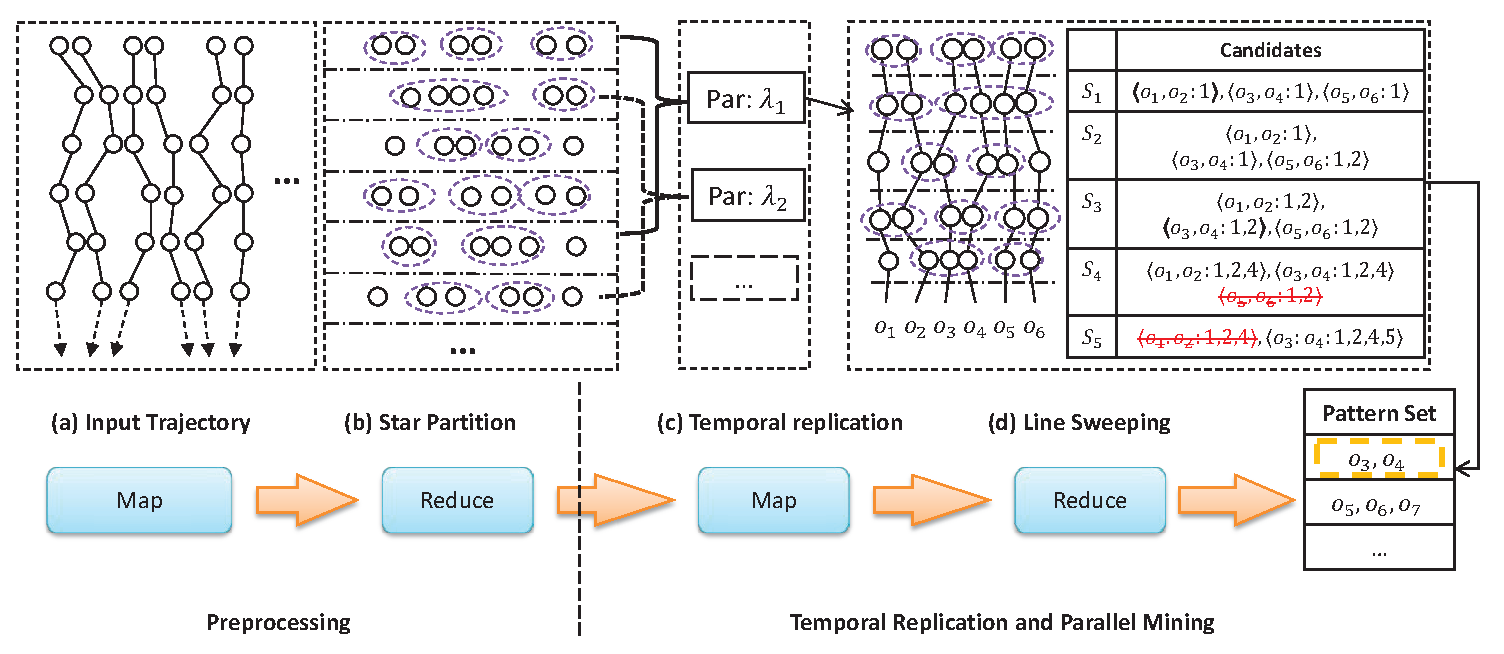
\includegraphics[width=\textwidth]{trm.eps}
\caption{Work flow of Temporal Replication and Mining. (a)(b) correspond to the first map-reduce cycle which clusters objects in each snapshot;  (c)(d) correspond to the second map-reduce cycle which uses temporal replication to mine GCMP in parallel.}
\label{fig:trm}
\end{figure*}








\emph{
Let $T$ be an arbitrary valid temporal sequence. Since $G$ equals to 1,
$T$ can be represented as $T=(t_1, t_2,...,t_m)$, where
$t_i +1 = t_{i+1}$ and $m \geq K$. Let $T' = (t_1,...,t_k)$, $T'$ is the shortest
valid temporal sequence of $T$. Note that $T'$ is fully contained
in the partition $\lambda_{t_1} = \{S_{t_1},...,S_{t_k}\}$, therefore it can be
mined in $\lambda_{t_1}$. 
Since $T$ is an arbitrary valid temporal sequence, the minimum $\eta$ is thus $K$.
}

Inspired by the observation, we generalize the relationship between
the minimum $\eta$ and temporal parameters using the following theorem:

\begin{theorem}
\label{THM:RP_ETA}
The minimum $\eta$ to ensure the completeness of the temporal replication is:
\[
   \eta = 
\begin{cases}
    (\lceil \frac{K}{L} \rceil -1)*(G-1)+2K -2, & \text{if } G \geq 2\\
    K,              & \text{if } G = 1
\end{cases}
\]
, where $K,L,G$ are the temporal parameters.
\end{theorem}

\begin{proof}
When $G = 1$, we have demonstrated $\eta=K$
in the above observation. When $G \geq 2$, we compute $\eta$ as follows:
any $T'$ can be viewed as $n$ consecutive segments with sizes $l_1,..,l_n$
and $n-1$ gaps with sizes $g_1,...,g_{n-1}$.
Since $\eta$ is the upper bond among all $T'$s, $\eta$ can be formulated 
as follows:
\begin{equation}
\eta = \max_{n,l_i,g_i} \{ \Sigma_{i=1}^{i=n} l_i + \Sigma_{i=1}^{i=n-1} g_i \}
\end{equation}
With the following constraints: (1)$\forall l_i, L \leq l_i \leq K-1$; (2)
$\forall g_i, 1 \leq g_i \leq G-1 $; (3) $\Sigma_{i=1}^{i=n} l_i \geq K$ and
(4) $\Sigma_{i=1}^{i=n-1}l_i  \leq K-1$. Constraints (1)(2)(3) due to the 
validity of $T'$ and $G\geq 2$ (4) is because $|T'|$ is minimum.
Based on (1)(3)(4), we can derive (5):  $n \in [1, \lceil \frac{K}{L} \rceil]$.
Constraints (1)-(5) form a convex polygon and $\eta$ is monotone
increasing wrt. $n, l_i, g_i$, therefore, the maximum value of $\eta$ is taken at the upper boundaries
where $g_i = G-1$, 
$\Sigma_{i=1}^{i=n-1}l_i = K-1$, $l_i = K-1$
and $n = \lceil \frac{K}{L} \rceil$. This leads to  $\eta = (\lceil \frac{K}{L} \rceil -1)*(G-1)+2K -2$.
\end{proof}

Based on the above theorem, during TRPM, every consecutive $\eta$ snapshots
form a partition. In particular, for every snapshot $S_t$, there is
a partition $\lambda_t=\{S_t,...,S_{t+\eta-1}\}$. With this partition strategy,
when discovering GCMPS in $\lambda_t$, we only need to keep the pattern candidates whose
object set are in $S_t$. This motivates to design an efficient 
\emph{line-sweep} mining (LSM) method for each partition. The intuition of LSM is 
to sequentially scan all snapshots. During scanning, a set of pattern candidates is maintained.
When all snapshots are scanned, the remaining candidates are the true patterns.
The detail of LSM is presented in Algorithm~\ref{algo:line-sweep}.
A candidate set $C$ is maintained throughout the algorithm(line~\ref{code:ls-can-set}). $C$
is initialized by inserting clusters at $S_t$ (lines~\ref{code:ls-init-start}-\ref{code:ls-init-end}).
During scanning snapshot $S_j$, candidates in $C$ are joined with clusters at $S_j$. In
the join, a candidate grows its temporal sequence while potentially reduces its object set. After the join,
false patterns are deleted (line~\ref{code:ls-remove}). 
Note that the size of $C$ is always decreasing, therefore the complexity of LSM $\lambda_t$ is $O(\eta|S_t||\overline{S}|)$,where $|\overline{S}|$ is the average snapshot size in $\lambda_t$.



\begin{algorithm}
\caption{Line Sweep Mining}
\label{algo:line-sweep}
\begin{algorithmic}[1]
\Require $\lambda_t = \{S_t, ..., S_{t+\eta-1}\}$
\State{$C \gets \{\}$} \Comment{Candidate set} \label{code:ls-can-set}
\For{$c \in S_t$} 
\label{code:ls-init-start}
\State $C$.add($\langle c, t \rangle $)
\EndFor
\label{code:ls-init-end}
\ForAll{$j \in [t+1,t+\eta-1]$}
\State $C \gets S_{j} \oplus C$ \label{code:ls-join}
	\State{remove false candidates from $C$}
	\label{code:ls-remove}
\EndFor
\State{output true candidates in $C$}
\end{algorithmic}
\end{algorithm}


%\begin{figure}[h]
%\centering
%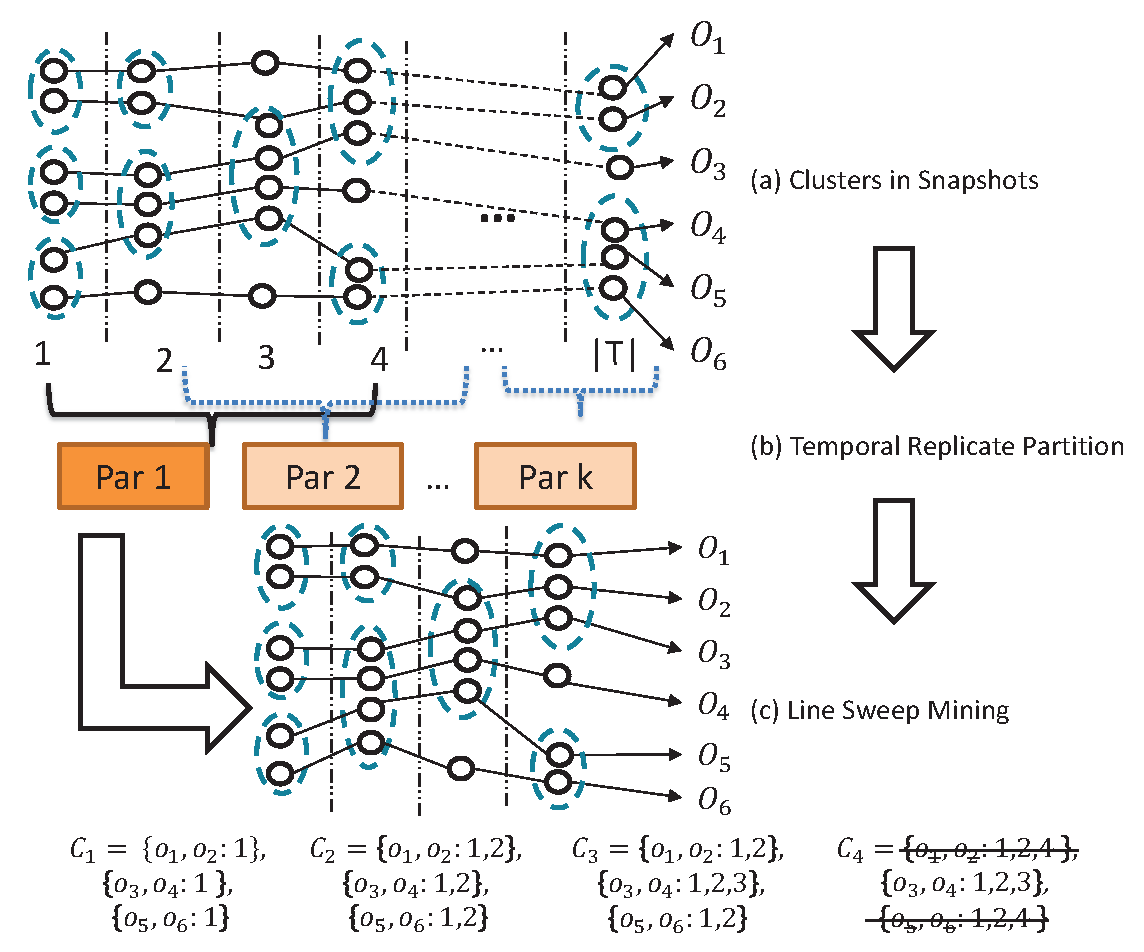
\includegraphics[width=0.5\textwidth]{trm_process.eps}
%\caption{Work flow of trajectory replication and mining}
%\label{fig:trm_process}
%\end{figure}


The complete picture of temporal replication and parallel mining is summarized in Algorithm~\ref{algo:trm_overview}. We illustrate the workflow of TRPM method using Figure~\ref{fig:trm} (c)(d) with pattern
parameters $M=2, K=3, L = 2, G=2$. By Theorem~\ref{THM:RP_ETA}, $\eta$ is calculated
as $(\lceil \frac{K}{L} \rceil-1) *(G-1)+2K - 2 = 5$. Therefore, 
in Figure~\ref{fig:trm} (c), every $5$ consecutive snapshots are combined 
into a partition in the map phase. In Figure~\ref{fig:trm} (d), a line sweep
method is illustrated for partition $\lambda_1$. Let $C_i$ be the candidate set
during sweeping snapshot $S_i$.
Initially, $C_1$ contains patterns whose object set is in snapshot $S_1$.
As line sweeps, the patterns in $C_i$ grows. At snapshot $S_4$, the candidate
$\{o_5,o_6\}$ is removed. This is because the gap between its latest timestamp (i.e., $2$)
and the next scanning timestamp (i.e., $5$) is $3$, which violates the $G$ constraint.
Next, at snapshot $S_5$, the candidate $\{o_1,o_2\}$ is removed. This is
because its local consecutive timestamps $\{4\}$ has only size $1$,
which violates the $L$ constraint.
Finally, $\{o_3,o_4\}$ is the qualified pattern and is outputted. Note that the minimum $\eta$
under this setting is $5$. If $\eta$ is chosen as $4$, the pattern $\{o_3,o_4\}$ would be excluded. 

\begin{algorithm}
\caption{Temporal Replication and Parallel Mining}
\label{algo:trm_overview}
\begin{algorithmic}[1]
\Require list of $\langle t, S_t \rangle$ pairs
\State $\eta \gets (\lceil \frac{K}{L} \rceil -1)*(G-1)+2K-2$
\State {---Map Phase---}
\label{code:trm-map-start}
\ForAll{$\langle t, S_t \rangle$}
	\ForAll{$i \in 1...{\eta-1}$}
		\State emit a $\langle \max(t-i,0), S_t \rangle$ pair
	\EndFor  
\EndFor
\label{code:trm-map-end}
\State {---Partition and Shuffle Phase---}
\label{code:trm-par-start}
\ForAll{$\langle t, S \rangle$ pair} 
\State group-by $t$, emit a $\langle t, \lambda_t\rangle$
\State where $\lambda_t = \{S_t, S_{t+1}, .. S_{t+\eta-1}\} $
\EndFor
\label{code:trm-par-end}
\State {---Reduce Phase---}
\label{code:trm-red-start}
\ForAll{$\langle t,\lambda_t \rangle$}
\State lineSweepMining($\lambda_t$)
\label{code:trm-red-end}
\EndFor
\end{algorithmic}
\end{algorithm}